\chapter{Case Study}\label{ch:case study}


\section{Problem}

\section{Company F}
For the validation of the OPS Framework company F was willing to participate in order to measure how agile are its teams. Company F \footnote{F is the first letter of the company's name} is a United States company which acts in the POS \footnote{Point Of Sales} area. With the development of some new products the company had a 300\% increase in the size of the development and QA departments resulting in the need for organizing better the development and release processes.

\subsection{Methodology F}
In general, company F does not follow a specific agile methodology, but rather a tailored mix of others which suit the needs of its team. 

Methodology F, as we can name it, embraces the following practices from the various agile methodologies \cite{koch2005agile}, some of the them in bigger and some of them in a smaller extent. \\

\begin{tabular}{| p{2cm} | p{13cm}|}
    \hline
     \textbf{Method} & \textbf{Practice} \\ \hline
     \textbf{XP}  & \begin{inparaenum} [a\upshape)]
     				\item Small Releases \item Simple design \item Refactoring \item Collective ownership \item Continuous integration \item 40-hour week \item Coding standards
					\end{inparaenum}      \\ \hline
     \textbf{FDD}  & \begin{inparaenum} [a\upshape)]  \item Developing by feature \item Feature teams \item Regular build schedule \item Inspections \item Configuration management
     				  \end{inparaenum}\\ \hline
     \textbf{Lean} & \begin{inparaenum} [a\upshape)] \item Empower the team \item Build Integrity In \item Amplify learning \item Eliminate waste
     				 \end{inparaenum} \\ \hline
\end{tabular}
\captionof{table}{Practices embraced in method F}


\subsection{Teams}
There are four development teams, each for a product of the company. Some of the teams have mixed members of developers and testers. In the Tables~\ref{table:teamA}, \ref{table:teamB}, \ref{table:teamC}, \ref{table:teamD}, one can see the structure of the teams. \\

\begin{minipage}[b]{0.45\textwidth}
  \centering
  \begin{tabular}{| p{3cm} | p{3cm}|}
    \hline
     \textbf{Team Size} & 7 \\ \hline
     \textbf{Roles}  & \begin{tabular}{@{}l@{}}Team Leader (1) \\ Developers (4) \\ Testers (3) \end{tabular} \\ \hline
     \textbf{Development Process}  & Method A \\ \hline
     \textbf{Area} & Mobile \\ \hline
     \textbf{Tools used}  & \begin{tabular}{@{}l@{}}Perforce \\ Titanium \end{tabular}  \\ \hline
     \textbf{Iteration length}  & 2-3 weeks \\ \hline
  \end{tabular}
  \captionof{table}{Team A - Profile} %Mobile
  \label{table:teamA}
\end{minipage}\qquad
\begin{minipage}[b]{.45\textwidth}
  \centering
  \begin{tabular}{| p{3cm} | p{3cm}|}
    \hline
     \textbf{Team Size} & 8 \\ \hline
     \textbf{Roles}  & \begin{tabular}{@{}l@{}}Team Leader (1) \\ Developers (5) \\ Testers (2) \end{tabular} \\ \hline
     \textbf{Development Process}  & Method B \\ \hline
     \textbf{Area} & Java \\ \hline
     \textbf{Tools used}  & \begin{tabular}{@{}l@{}}Perforce \\ Eclipse IDE \end{tabular} \\ \hline
     \textbf{Iteration length}  & 2-3 weeks \\ \hline
  \end{tabular}
  \captionof{table}{Team B - Profile} %Marketing
  \label{table:teamB}
\end{minipage}



\begin{minipage}[b]{0.45\textwidth}
  \centering
  \begin{tabular}{| p{3cm} | p{3cm}|}
    \hline
     \textbf{Team Size} & 4 \\ \hline
     \textbf{Roles}  & \begin{tabular}{@{}l@{}}Team Leader (1) \\ Developers (1) \\ Testers (2) \end{tabular} \\ \hline
     \textbf{Development Process}  & Method C \\ \hline
     \textbf{Area} & Java \\ \hline
     \textbf{Tools used}  & \begin{tabular}{@{}l@{}}Perforce \\ Eclipse IDE \end{tabular}  \\ \hline
     \textbf{Iteration length}  & 2-3 weeks \\ \hline
  \end{tabular}
  \captionof{table}{Team C - Profile} %Info
  \label{table:teamC}
\end{minipage}\qquad
\begin{minipage}[b]{.45\textwidth}
  \centering
  \begin{tabular}{| p{3cm} | p{3cm}|}
    \hline
     \textbf{Team Size} & 17 \\ \hline
     \textbf{Roles}  & \begin{tabular}{@{}l@{}}Team Leader (1) \\ Developers (9) \\ Testers (7) \end{tabular} \\ \hline
     \textbf{Development Process}  & Method D \\ \hline
     \textbf{Area} & Java \\ \hline
     \textbf{Tools used}  & \begin{tabular}{@{}l@{}}Perforce \\ Eclipse IDE \end{tabular} \\ \hline
     \textbf{Iteration length}  & 2-4 weeks \\ \hline
  \end{tabular}
  \captionof{table}{Team D - Profile} %POS
  \label{table:teamD}
\end{minipage}

%analyze more what each team does


\section{Method}

\subsection{Introduction}
In order to measure the adequacy, the capability and the effectiveness of methodology F, the described method by \citet{sventha_dissertation} was followed.

\subsection{Scales}

\begin{minipage}[b]{0.25\textwidth}
  \centering
  \begin{tabular}{| c | c |}
 \hline
 \textbf{Answer} & \textbf{Score} \\ \hline
 Yes/Fully & 5 \\ \hline
 Partiallty & 3 \\ \hline
 No/Marginally & 1 \\ \hline 
\end{tabular}
\captionof{table}{Scale for Capability}
\end{minipage}\qquad
\begin{minipage}[b]{.3\textwidth}
  \centering
  \begin{tabular}{| c | c |}
 \hline
 \textbf{Answer} & \textbf{Score} \\ \hline
 Maximally & 5 \\ \hline
 Considerably & 5 \\ \hline
 Moderately & 3 \\ \hline
 Somewhat & 2 \\ \hline
 Marginally & 1 \\ \hline 
\end{tabular}
\captionof{table}{Scale for Effectiveness}
\end{minipage}
\begin{minipage}[b]{.35\textwidth}
  \centering
\begin{tabular}{| c | c |}
 \hline
 \textbf{Score Range} & \textbf{Interpretation} \\ \hline
 4.5 - 5.0 & Maximal \\ \hline
 3.5 - 4.4 & Considerable \\ \hline
 2.5 - 3.4 & Moderate \\ \hline
 1.5 - 2.4 & Somewhat \\ \hline
 1 - 1.4 & Marginal \\ \hline 
\end{tabular}
\captionof{table}{Scale for intrepreting final scores}
\end{minipage}

\subsection{Assessing the Adequacy}

In order to assess the adequacy a top down approach was followed for each objective, principle and strategy as it is described by \citet{sventha} %add reference to the figure too}.
 For the analysis of each objective, principle and strategy the analysis of agile methodologies based on \citet{koch2005agile} was followed.

Initially the objectives fulfilled by methodology F were identified. As it can be seen in Figure~\ref{fig:companyF_objectives} all five objectives mandated by the OPS Framework are followed.

\begin{figure}[H]
\centerline{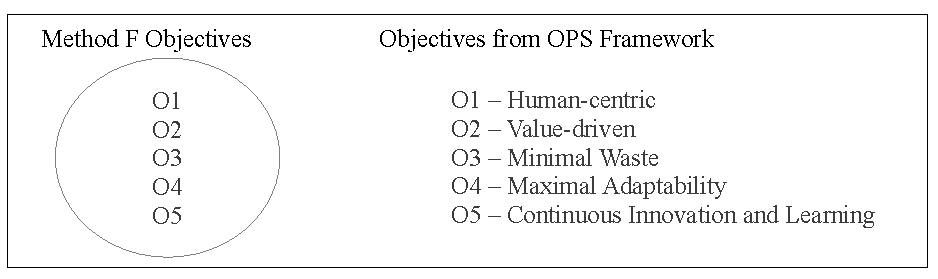
\includegraphics[scale=0.9]{include/case_study/fig/companyF_objectives.pdf}}
\caption{Objectives identified in methodology F} 
\label{fig:companyF_objectives}
\end{figure}

Based on the objectives and following the linkages from them the principles were identified. As one can see in Figure~\ref{fig:companyF_objectives} methodology F does not follow the ``Frequent Reflection and Improvement" principle because the organization rarely does it re-examine the development process in order to improve it. %maybe justify why!
It is worth mentioning that the ``Empowering teams of Motivated Individuals" principles is not entirely followed, but it differs among the teams. Every team is built with motivated individuals, some to a more and some to a lesser extent. 

\begin{figure}[H]
\centerline{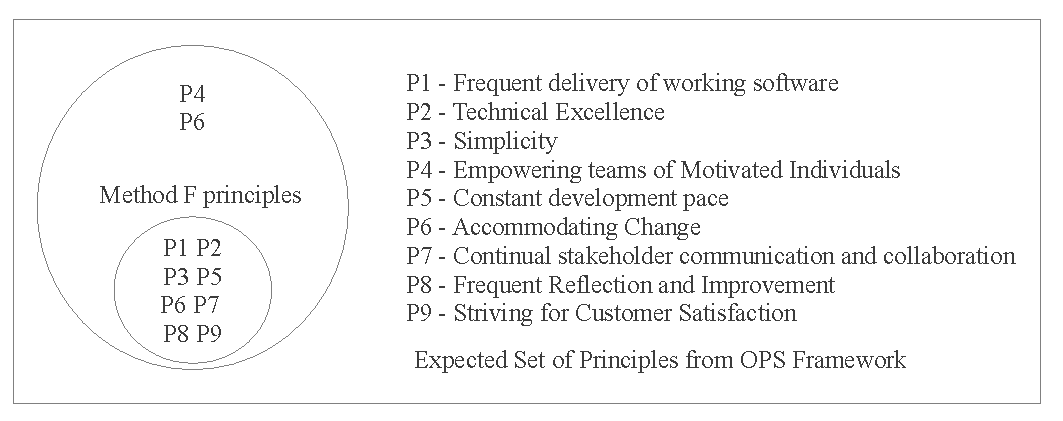
\includegraphics[scale=0.9]{include/case_study/fig/companyF_principles.pdf}}
\caption{Principles identified in methodology F} 
\label{fig:companyF_principles}
\end{figure}

Following the linkages from the principles the strategies for implementing them were identified. As it can be seen in Figure~\ref{fig:companyF_strategies} methodology F does not support 

\begin{itemize}
\item \textbf{Continuous feedback} - The organization does not have a defined process for getting a feedback from the customers of the company. From time to time the managers of the various departments of the company have personal conversations with the customers. If any issue arises, then they inform the development and QA departments in order to identify the problem and fix it.
\item \textbf{Test-first development} - None of the team members writes tests before starting coding.
\item \textbf{Constant velocity} - The organization does not measure the velocity of the teams. In general the pace of development and integration and deployment is based on the needs of the customers and the capability of the developer. No one has to finish a specific amount of work in each iteration. What is only wanted, is the functionality to be ready when it is scheduled.
\item \textbf{Retrospection} - Although there is a tendency to change this, the teams do not have a process for retrospection. The team members unconsciously consider that they are doing fine, unless a team leader or the manager of the department tells them the opposite.
\end{itemize}

\begin{figure}[H]
\centerline{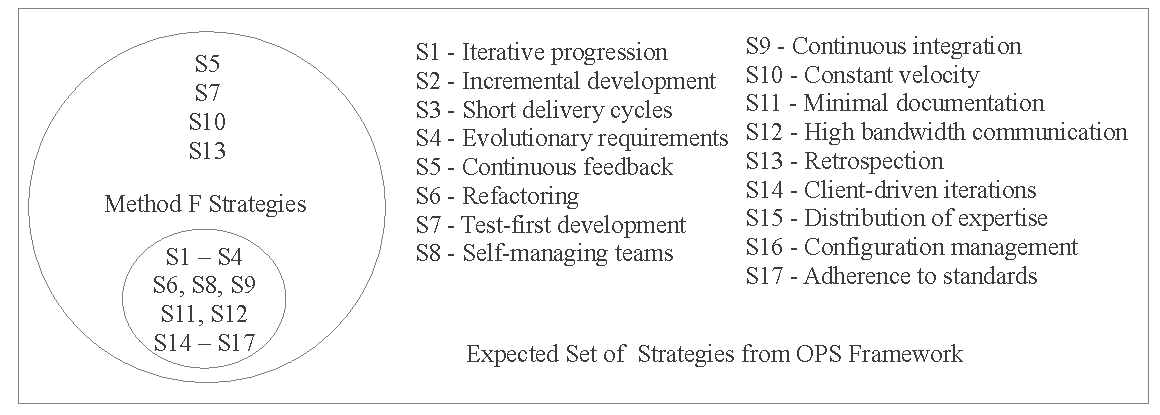
\includegraphics[scale=0.9]{include/case_study/fig/companyF_strategies.pdf}}
\caption{Strategies identified in methodology F} 
\label{fig:companyF_strategies}
\end{figure}

%Analyze more the adequacy
Reflecting on the above analysis, we see that methodology F lacks four strategies which are important for its improvement. Without retrospection the team members do not always identify and discuss their mistakes, while without a well defined process for continuous feedback any issues that might arise may go unnoticed for quite some time. In total, methodology F is missing four strategies out of seventeen which is a lot. As a result the adequacy of the methodology is questionnable.



\subsection{Team A}
\subsubsection{Capability Assessement}
\subsubsection{Effectiveness Assessement}

\subsection{Team B}
\subsubsection{Capability Assessement}
\subsubsection{Effectiveness Assessement}

\subsection{Team C}
\subsubsection{Capability Assessement}
\subsubsection{Effectiveness Assessement}

\subsection{Team D}
\subsubsection{Capability Assessement}
\subsubsection{Effectiveness Assessement}


%~\nameref{sec:capability_hierarchy}






\section{Results}

\section{Discussion}
